\chapter{Introduction}

%The story  I want to tell explains the Casimir force via its historical origins which serve to introduce the big results, while sidestepping weird irrelevant bullshit.  I want to hit the important context for modern scientists and emphasize quantities realted to current experiments.  I also want to outline the currently available most powerful methods to set context for what else is possible, and what its limitations are.  

%I think I can do this with a partial historical introduction.

Quantum mechanics is an inherently statistical theory - we can only make predictions for the probabilities of events.  
\comment{Cite Dirac/Sakurai as general textbook}.
\begin{itemize}
\item Add complex amplitudes together.  Take modulus squared to get probabilities.  
\item Feynman path integral construction of quantum mechanics- to get amplitude to get from one position to another, add up \emph{all} possible paths, with a suitable phase, $e^{-i S[x]/\hbar}$, \cite{Feynman1942, Feynman1965}
\item Found common use in field theory particularly for covariantly quantizing gauge field theories, such as the Standard Model (cite Weinberg).  Integrate over all field configurations.  
\item  Also related to stochastic processes, like Brownian motion \cite{Karatzas1991}.   Can mathematically formulate a path integral as very high-dimensional integral.  Can then use Monte-Carlo methods, to randomly sample from most important regions of integral.  
\end{itemize}

\begin{itemize}
\item Quantum measurements are inherently probabilitistic.  
\item Thus, sequences of measurements are also inherently random.  
\item Greater experiemtnal control means we can now probe isolated quantum systems repeatedly and see how they evolve.  
\item Move beyond simple projective measurements, which cannot describe things like position measurements.
\item To describe continuously weakly probing a system, also use stochastic processes as part of numerical simulation strategy.
\item Quantum tajectories correspond to monitoring a quantum system (like an atom) via a probe, for example shining light on the atom. \cite{Carmichael1993}
\item Simulated trajectories are possible trajectories a system could trace out as we observe.  Also given a particular measurement record, they correspond to our best estimate of the current state of the system.  
\end{itemize}

\comment{There are two roles for the randomness here.  From one point of view, the randomness is an intrinsic part of quantum mechanics, and thus naturally shows up in fluctuation phenomena like the Casimir effect, or in quantum measurements.  Alternatively, if we are considering these calculations for energy or evolution as large integrals, then we can efficiently compute these integrals by randomly sampling from their dominant regions.  In this sense, the randomness shows up as a calculational tool.}

This thesis will cover a two different computational projects in quantum optics.
The first project relates to computing Casimir forces via the worldline method.
  Most of the thesis is devoted to discussing the background, 
and discussing the analytical and numerical techniques developed.
  In brief, the worldline method is a numerical method for computing Casimir energies via path integrals.
  The numerical simulations

The second theme will be using quantum trajectories to simulate continupus positions measurements on atoms.
Both of these projects are related to fundamental quantum optical phenomena, 
that we will explore using stochastic calculus, and Monte-Carlo methods for numerical simulations.  

\begin{itemize}
\item General thesis about quantum physics of atoms using computation.  
\item Thesis covers numerical monte-carlo techniques, where random numbers used in simulation.
\item First new method for computing electromagnetic Casimir energies.
\item Second, continuous position measurements of atoms taking into account experimental constraints.  
\item United in perspective of numerical work relying on Monte-Carlo techniques, to explore quantum phenomena relevant to modern experiments and pushes toward future technology  
\end{itemize}



\section{Casimir Forces in general and physical interpretation}

\begin{itemize}
\item Casimir force arises due to fluctuations in quantum fields. 
\item Forces between macroscopic bodies, atoms and bodies and between atoms.  
\item Interesting for theory reasons as purely quantum field theory phenomena, 
  and relevance to current experimental physics.  
\end{itemize}


\begin{itemize}
\item General references Cite Books - Milonni~\cite{Milonni1994}, Milton~\cite{Milton2001}.
  Bordag~\cite{Bordag2009}, Dalvit~\cite{Dalvit2011} recent developments.  
\item More general books on Casimir and van der Waals forces as they relate to chemistry, 
  Parsegian~\cite{Parsegian2006}, Israelachivili~\cite{Israelachvili2011}.
\end{itemize}


\subsection{Casimir energy}

The Casimir force is an force that arises between bodies due to fluctuations in quantum fields.
  It was first predicted in 1948 by Henrik Casimir~\cite{Casimir1948}.
  If we consider two planar perfect conductors, we find that there is an 
attractive force between them due to the zero point energy of the electromagnetic field.
  In a quantum electrodynamics the ground state of each mode of the 
electromagnetic field contributes $\hbar\omega/2$, where $\hbar$ is Planck's
 constant, and $\omega$ is the frequency of the mode.
  The presence of the conductors forces the electric field to vanish on the surfaces,
 which restricts the allowed modes of the electromagnetic field.  
If we add up the energy from all modes of the electromagnetic field, 
and compare it to the case when the plates are infinitely far apart from one another, 
we find the energy is reduced as the plates are brought closer together.

  The energy between the plates is then
\begin{equation}
  E = -\frac{\hbar c}{240\pi^2 d^3},
\end{equation}
where $c$ is the speed of light in vacuum, $\hbar$ is the reduced Planck constant,
and $d$ is the distance between the plates.  

\subsubsection{Calculation for perfect conductors}

\comment{Give simple derivation of force? Cite Bordag/Dalvit?}
Here we will briefly reprise Casimir's original calculation~\cite{Casimir1948}.
  Let us consider a perfectly conducting box of length $L$.
  We will place another perfectly conducting plate, of area $L^2$, a distance $a$ from the $xy$ wall.   
If we consider the quantized electromagnetic field,  
then the energy of the field in its ground state is
\begin{equation}
E = \sum_{\text{modes}}\frac{\hbar\omega_\alpha}{2}.
\end{equation}
Since the energies for each mode are positive, and the sum extends over all possible modes,
 this enery is extremely divergent.
  However, if we consider energy \emph{differences} between two configurations 
we can find a finite result.  
This subtraction is a form of renormalization.  

We can write down the allowed modes for a rectangular cavity defined by, 
\begin{equation}
0 \le x \le L, \quad 0 \le y\le L, \quad 0 \le z \le a.
\end{equation}
From the boundary conditions, and transversality of the field,
 the mode functions for a perfectly conducting box 
are\footnote{Eq. (8.62) in `` Quantum and Atom Optics'', by Daniel A. Steck 
\cite{SteckQuantumOptics}}:
\begin{align}
\mathbf{f}_{\mathbf{k},\zeta}(\mathbf{r}) =& \sqrt{\frac{8}{V}}\bigg[ \hat{x}(\hat{\epsilon}_{\mathbf{k},\zeta}\cdot\hat{x})\cos k_xx\sin k_yy\sin k_z z\nonumber\\
&+\hat{y}(\hat{\epsilon}_{\mathbf{k},\zeta}\cdot\hat{y})\sin k_xx\cos k_yy\sin k_z z\nonumber\\
&+\hat{z}(\hat{\epsilon}_{\mathbf{k},\zeta}\cdot\hat{z})\sin k_xx\sin k_yy\cos k_z z\bigg],
\end{align}
where $\hat{\epsilon}_{\mathbf{k},\zeta}$ is the polarization vector associated with
 the mode with wavevector $\vect{k}$ and the polarization index $\zeta$ takes on two values.
  The conducting boundary conditions mean that the fields must vanish on the surfaces, which requires that
\begin{equation}
k_x = \frac{pi n_x}{L},\quad  k_y = \frac{\pi n_y}{L}, \quad k_z=\frac{\pi n_z}{a},
\end{equation}
where $n_x,n_y,n_z$ are positive integers. 
 The requirement that $\nabla\cdot\vect{E}=0$, then requires that 
$\vect{k}\cdot\vect{E}=0$, which limits the polarizations to two values.
  We can write the frequency for a particular mode as
\begin{equation}
  \omega = c|\vect{k}| = c\sqrt{k_x^2+k_y^2+k_z^2}.
\end{equation}
Then if we take the limit $L\rightarrow\infty$, we can replace the sums over
 these modes with integrals over a continuum, 
\begin{equation}
E = \hbar c\bigg(\frac{L}{\pi}\bigg)^2{\sum_{n_z=0}^\infty}'\int_0^\infty dk_x
\int_0^\infty dk_y \left(\sqrt{k_x^2+k_y^2+\frac{n_z^2\pi^2}{a^2}}\right),
\end{equation}
where ${\sum_n}'$ includes a factor of $1/2$ for the $n=0$ term.
  (At $n_z=0$, there is only one polarization, while for larger $n$ there are 
two polarizations.  
When we come to consider non-zero temperature effects later, 
we will encounter similar summations.)

We can introduce polar coordinates to evaluate the integral over $k_x,k_y$.  
If we define $\kappa=\sqrt{k_x^2+k_y^2}$, and carry out the angular integral in 
the upper quarter plane, we find
\begin{equation}
E = \hbar c\bigg(\frac{L}{\pi}\bigg)^2\frac{\pi}{2}{\sum_{n_z=0}^\infty}'
\int_0^\infty d\kappa\,\kappa \sqrt{\kappa^2+\frac{n_z^2\pi^2}{a^2}}.
\end{equation}

On its own this energy is highly divergent.  
We will then subtract off the energy when the plates are moved farther apart.
In the limit of large $a$ we can also convert the sum over integers into 
another integral.  
The result of this subtraction is
\begin{equation}
E = \hbar c\bigg(\frac{L}{\pi}\bigg)^2\frac{\pi}{2}\int_0^\infty d\kappa\,\kappa
 \left({\sum_{n_z=0}^\infty}'\sqrt{\kappa^2+\frac{n_z^2\pi^2}{a^2}}
-\frac{\pi}{a}\int_0^\infty dk_z\sqrt{\kappa^2+k_z^2}\right).
\end{equation}
At this point Casimir introduces a function $f(k/k_m)$ to regularize the calculation.
This physically amounts to including some dispersion to model an 
ultra-violet (UV) cutoff.  
It is known \comment{Kramers-Kr\"onig} that the metal becomes transparent to 
photons at high enough energies, or short enough wavelengths,
 where $k_m$ indicates the cutoff.
  $f(k/k_m)$ is one for $k\ll 1$, and approaches zero for $k\gg k_m$.  

If we change variable again to $u=(a\kappa/\pi)^2$, then
\begin{equation}
E = \hbar c\bigg(\frac{L}{\pi}\bigg)^2\frac{\pi}{2}\frac{1}{2}
\left(\frac{\pi}{a}\right)^3\int_0^\infty du 
\left({\sum_{n_z=0}^\infty}'\sqrt{u+n_z^2}-\frac{\pi}{a}\int_0^\infty dn\sqrt{u+n^2}\right)
f\left(\frac{\pi\sqrt{n^2+u}}{a k_m}\right).
\end{equation}
%(\pi/a)^2 \frac{1}{2} from change of variable
If we now use the Euler-Maclaurin formula,
\begin{equation}
{\sum_{n=0}^\infty}' F(n)-\int_0^\infty dn\, F(n)
=-\frac{1}{12}F'(0)+\frac{1}{24\times 30}F'''(0),
\end{equation}
where primes denote differentiation w.r.t the argument, 
\begin{equation}
F(n)=\int_{n^2}^\infty dw\, \sqrt{w}f\left(\frac{\pi w}{ak_m}\right),
\end{equation}
where we have changed variables in the $u$ integral to $w = \sqrt{n^2+u}$
Then taking 
\begin{align}
F'(n) & = -\frac{2n^2}f\left(\frac{\pi n^2}{a k_m}\right)\\
F'(0) & = 0\\
F'''(0) & = -4
\end{align}
\comment{huh?  Introduced $f(k)$ to regularize Euler-Maclaurin}.

The end result of this, this that the renormalied vacuum energy per unit area is
\begin{equation}
\frac{E}{L^2} = -\frac{\hbar c\pi^2}{720 a^3}
\end{equation}

\begin{figure}
\center
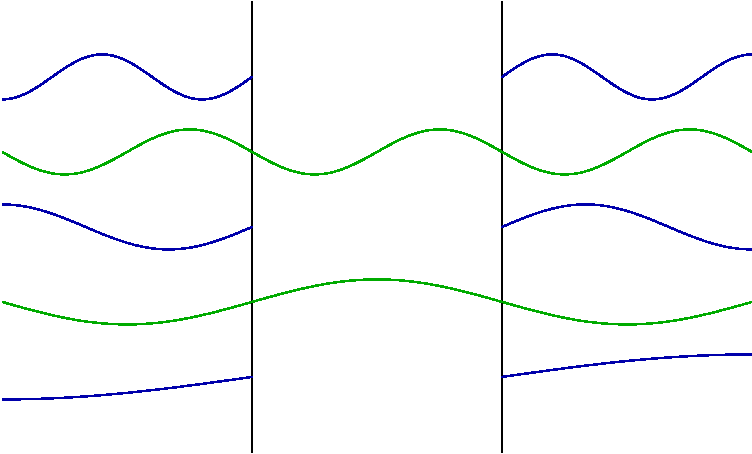
\includegraphics[width=10cm]{fig/intro/twoplanes_wave}
\caption{Sketch of allowed modes between perfectly conducting plates.}
\end{figure}


This example calculation is also carried out in the initial chapters of Ref.s~\cite{Milton2001,Bordag2009,Dalvit2011}.





\subsection{Casimir-Polder energy}

The Casimir force is also important for atoms near surfaces.  
This variant is known as the Casimir-Polder force, 
after a paper by Casimir and Polder where they computed the force between an 
atom and a perfect conductor accounting retardation due to the finite speed 
of light~\cite{CasimirPolder1948}.  
In this case, the atom feels an attractive potential to a surface a distance $d$ away,
\begin{equation}
V_{CP} =-\frac{3\hbar c\alpha_0}{64\pi^2\epsilon_0 d^4}.
\end{equation}

\comment{Note Dan's notes as example calculations.  }

\subsection{Van der Waals forces}

The formalism was extended to include dielectric media by Lifshitz~\cite{Lifshitz1956}.
  \comment{He also worked alongside co-workers Dzayolshinkii and Abrisokov to
 further compute the force from using Feynman diagrammatic methods\cite{Dzyaloshinskii1959,Dzyaloshinskii1961}}.  
\comment{Point of view: Due to thermal fluctuations in medium.}

\comment{Mclachlan\cite{Mclachlan1963} cites these guys?}


\subsection{Scale and Physical Interpretation}

\begin{itemize}
\item Ground state energy or zero point enery.  
Emphasizes boundary conditions and restricted spectrum of fluctuations.  
\item Atoms emitting and absorbing virtual photons.  
\item Feynman Diagram.  
Atom-Wall
\begin{figure}
  \centering
\begin{fmffile}{atom-loop}
  \begin{fmfgraph*}(100,60)
    \fmfleft{i}
    \fmfright{o}
    \fmftop{t}
    \fmf{plain}{i,v1}
    \fmf{plain}{v2,o}
    \fmf{plain,label=$|e\rangle$}{v1,v2}
    \fmf{photon,left=0.5,tension=.4}{v1,vt,v2}
    \fmf{phantom,tension=1}{t,vt}
    \fmflabel{$|g\rangle$}{i}
    \fmflabel{$|g\rangle$}{o}
    \fmflabel{$\gamma$}{vt}
  \end{fmfgraph*}
\end{fmffile}
\caption{Atom interacting with wall via emitting and absorbing photons.  }
\end{figure}

Wall-Wall Effective action.

\begin{figure}
\centering
\begin{fmffile}{wall-wall}
\begin{fmfgraph}(50,30)
 \fmftop{t0,t1,t2,t3}
 \fmfbottom{b0,b1,b2,b3}
 \fmf{phantom}{t1,v1}
 \fmf{phantom}{t2,v3}
 \fmf{phantom}{b1,v2}
 \fmf{phantom}{b2,v4}
 \fmffreeze
\fmf{photon}{v1,v3}
\fmf{photon}{v2,v4}
\fmf{fermion,tension=0}{v1,v2}
\fmf{fermion,tension=0,left}{v2,v1}
\fmf{fermion,tension=0}{v3,v4}
\fmf{fermion,tension=0,right}{v4,v3}
\end{fmfgraph}
\end{fmffile}
\caption{Casimir Energy in terms of fundamental QED processes.  Electrons are considered bound within their respective media.}
\end{figure}

\item Picture of Electrons interacting with EM field.
  Effective action at some loop order in basic QED.
  Makes contact with fundamental physics.
  Can then make sense of limits in which we are operating.
  Doing perturbation theory on QED.
  $\epsilon$ is linear response of medium to EM field, and working to leading order in $\epsilon$.
  Amounts to $\order(\alpha_0^4)$ diagram for QED with electrons bound via nuclear potential.   (Again, very low energies).
\begin{itemize}
\item Assuming electrically neutral
\item Far from atomic separations, so continuum approximation acceptable.
\end{itemize}

\item Casimir forces are short ranged forces and decay away quickly.
  The Coulomb potential between charged particles is behaves as $d^{-1}$,
 where $d$ is the particles separation.
  In comparison, the London dispersive force between two atoms decays as $d^{-7}$.
  For macroscopic bodies, the decay is slower, since we can roughly think of
 adding up the contributions from all of the constituent atoms.
  For Casimir energies, the energy decays as $d^{-3}$.  

These considerations are for zero temperature.
  It turns out that considering the effects of finite temperature, 
in particular thermal photons, leads to different distance dependence again.
  The energies typically decay more slowly in the high temperature limit.
  If the Casimir force decays as $d^{-n}$ at zero temperature, 
then we typically find that the force decays as $r^{-n+1}$ at high temperatures.  

We can estimate typical distance scales by considering the dominant 
resonances of the medium, and the thermal wavelength.
  So the Casimir force is typically then important at distances below the
 transition wavelength which is usually around $1\mu m$.    

\item The typical energy scale can also be estimated.
  If we consider an atom with a static polarizability of 
$\comment{polarizability}$, at a distance of $1\mu m$, we find the Casimir-Polder potential is \ldots. 

For macroscopic bodies we can compare the Casimir energy for perfect 
metal conductors at a distance $d$ to the energy stored in the capacitance.
  Note that we compute an energy per unit area.  
\comment{Milonni makes the comparison to capacitance, \cite{Milonni1994}}

The Casimir energy per unit area is $\frac{\hbar c\pi^2}{240 d^3}$, while the voltage for a parallel plate capacitor is.
\begin{shaded}
\begin{itemize}
\item Capacitance is $V=Q/C$.  
\item $C = \epsilon_0 A/d$.  
\item Energy is $\frac{1}{2}CV^2=\frac{Q^2}{2C} $
\end{itemize}
\end{shaded}

\end{itemize}


\begin{itemize}
%\item Cite Casimir/Casimir-Polder and Lifshitz.
\item Casimir vs Van Der Waals vs London Forces

The Casimir force is intimately related to the van der Waals forces between molecules.
Van der Waals forces are usually ascribed to the dipole fluctuations of the 
neutral atoms.
In the limit where the atoms are far apart retardation becomes important and 
the force changes decays more quickly as $r^{-7}$.
  In this limit the forces are sometimes referred to as London dispersion forces.
  Normally Casimir forces consider the 

Throughout this thesis we shall use Casimir forces to refer to the forces between
 macroscopic bodies, and Casimir-Polder forces to refer to the forces between 
atoms and macroscopic bodies.  

\item Renormalization

As QED calculation, the Casimir energy is formally divergent and must be renormalized. 
 In our case, we typically energy differences when one of the bodies is 
removed to spatial infinity.
  In some cases, like spheres we must consider renormalization more carefully.
  In those cases, the formally infinite parameters we get renormalize the 
physical parameters of the model~\cite{Milton2001}.  

\item Non-additivity of forces:  Reference for this?  What is the typical scale of the correction for non-additivity?

\item Search for repulsive forces

\begin{itemize}
\item Casimir force important for stiction.
\item Attracts atoms, sets lower bound for how close you can get particles together.
\item Search for repulsive forces as possible trapping (Motivation for this?)
\item Can be found for magnetic media (but typically small).
  Metamaterials exhibit this for small range of frequencies.
  But Casimir broadband, and dielectric contribution ends up dominating.
  (\comment{ Cite Milonni on metametarials}.
Sufficiently anistropic dielectric media (how anisotropic? \comment{Cite Milton})
 $\epsilon_1<\epsilon_3<\epsilon_2$ over a broad enough range of frequencies 
\comment{Cite Lifshitz of liquid helium.
  Cite experiments, and note odd fluids.}.
   Geometries dependence (\comment{Cite reid paper on needle above hole}).
\end{itemize}
\item Dynamical Casimir effect/Unruh Effect?
\begin{itemize}
  \item Accelerating plate creates photons.  L
\end{itemize}
\end{itemize}

\subsection{Worst prediction in physics}

Let us briefly note that the Casimir energy is sometimes related to the cosmological constant in general relativity.
  ``one of the worst predictions in physics.''  
In Einstein's General Theory of Relativity, energy is coupled to the metric of spacetime.
  The cosmological constant acts to drive accelerating expansion~\cite{Carroll2004}.
  Note that the cosmological constant can be provided by the vacuum energy of the quantum fields of matter on spacetime.
  Note however that it is the energy itself that shows up, not energy differences. 
If we attempt to identify the vacuum energy with the cosmological constant, we estimate the energy from 
\begin{equation}
E \sim \int_0^\Lambda dk\,k^2 (\hbar c k),
\end{equation}
where $\Lambda$ is a high-frequency cutoff, which denotes the short wavelength
 below which our effective description of the world in terms of quantum 
field theory breaks down.
  If we pick $\Lambda=[c^3/(\hbar G)]^{1/3}$ to be the Plank wavelength, 
where $G$ is Newton's gravitation constant, at which point quantum gravity
 effects are expected to become important, then we predict, 
\begin{equation}
E \sim \hbar c \Lambda^4 
\end{equation}
Unfortunately, this is around $10^{120}$ times too large relative to the 
measured value.  T
his discrepency is known as the cosmological constant problem.  
Fortunately, we will always be considering experiments on a more terrestrial scale,
 where it makes much more physical sense to only consider energy differences.
  In which case, these issues do not arise, and experiments and theory are in much closer accord.    


\section{Physical relevance and experimental relevance}

\section{Experiments}
\subsection{Physics}
\begin{itemize}
\item Liquid Helium
\item Spaarnay

\item Lamoreaux - for 1997 measurements\cite{Lamoreaux1997}, and also recent thermal work by Sushkov\cite{Sushkov2011}.

\item Mohideen \cite{Mohideen1998} AFM with sphere above plate.

\item Capasso \cite{Chan2001}  torsion oscillator above plate
\item Bressi \cite{Bressi2002} Parallel Plates.
\item Sukenik\cite{Sukenik1993}, atoms passing through cavity to detect Casimir-Polder.  
\item Cornell - atoms near wall\cite{Harber2005, Obrecht2007}.
  BEC near wall, detect change in oscillation frequency of trap due to Casimir-Polder energy.
  Using thermal shift?
\item Antezza - chapters in Dalvit.  
\item Kimble atoms near toroidal resonators.
  \cite{Alton2011}.
  Atoms above 1D Microcavity \cite{Hung2013}
\item Atom-chips  Schmiedmeyer\cite{Folman2000,Schneider2003}(?)  Not explicitly using Casimir-Polder forces?  
\item Cronin \cite{Perreault2005,Lonij2009}  Atom interferometry experiments for atoms near gratings.
\end{itemize}

\begin{itemize}
\item Controversies about role of zero temperature pole.  
\item Lamoreaux favors Drude model, Capasso favours plasma model.
\item Seems experiments favour more 
\end{itemize}

\subsection{Chemistry/Helium/Geckos?}

\begin{itemize}
\item Geckos use the Casimir force \cite{Autumn2002}.
\end{itemize}

\subsection{Modifications to gravity}

\begin{itemize}
\item Modifications to gravity on $1\mu m$ or $1mm$ scale.  Cite Lamoreaux 2000 Paper.  Gervaci?
Yukawa type forces.  
\item Subtract off Casimir force background.
  Tino group.
  Use Casimir shield with fairly thick gold to have same Casimir force, and thne vary the medium behind it.
  Longer range gravity should lead to 
Requires very careful measurements, on top of carefully extracting Casimir force.   
\end{itemize}

\section{Other Computational methods}

\subsection{Proximity Force Approximation}

\begin{itemize}
\item Find first use?  Lamoreaux mentions usage.  Derjaguin?\cite{Derjaguin1956}
\item Note problem with non-additivity. 
\item Good as order of magnitude estimate?  
Useful if very limited curvature, or effectively approximate geometry as planar.  
\end{itemize}

\subsection{Green function methods}

\begin{itemize}
\item Cite Schwinger~\cite{Schwinger1978, Milton1978}  Scalar green functions.  
\item Green tensor methods
\item Cite Barton
\item Cite Philbin(?)
\item Cite Vogel and Welsch
\end{itemize}

\subsection{Reflection Matrix}

\begin{itemize}
\item Cite Balian and Duplantier \cite{Balian1977, Balian1978}.
\item Cite Lambrecht and French collaborators
  \cite{Lambrecht2006, MaiaNeto2008,Canaguier-Durand2012}
\item Cite Milton
\end{itemize}

\subsection{Scattering Matrix Path Integral Methods}

\begin{itemize}
\item Physical Picture based on generalized Green theorem from 
  SIE~\comment{Stratton}\cite{Stratton1941}.
\begin{itemize}
\item What are the SIE ?  
\item Comment on Emig/Buscher showing you can use homogenous green function.
  Relation to Green's theorem.
\end{itemize}

\item Cite Emig,Jaffe,  and others for initial analytical techniques.  Relies on Green theorem.
\cite{Emig2004, Emig2007, Rahi2009}
\item Cite Johnson/Reid/ for numerical progress.
  Note use of existent analytical methods and similarities to existent 
numerical FTDT techniques on earlier papers.  \cite{Reid2009,Reid2011, Reid2013} 
\cite{Rodriguez2007,Rodriguez2007a, Rodriguez2009}
\item Note success, applicability.  \comment{Cite experimental tylenol pill paper}
\item Estimates on scaling of algorithm?
\end{itemize}

\subsection{Worldlines}

The worldline method is an alternative method for computing Casimir energies.
  The worldline method was initially developed as an alternative method for 
carrying out QFT calculations in terms of particle 
mechanics~\cite{McKeon1993, Strassler1992,Schubert2001}.
  In particular we can compute compute quantum effective actions in terms of
 the suitable dynamics of a quantum particle.
\comment{Other references - was one contemporaneous with Strassler? Bern-Kosower}

The basic insight is that for one loop effective actions, 
we can recast a field path integral calculation in terms of the particle path
 integral for particles travelling in closed space-time loops.
  This is quite similar to the scalar electrodynamics Feynman explored
 in his Ph.D thesis~\cite{Feynman1942, Brown2005}
\comment{Seems to actually be his 1950 QED paper RE Schubert2001}.
  Higher order loop calculations can also be carried out with more particles, 
and gauge fields can also be treated~\cite{Schubert2001}.
  For example, the worldline method has been used to compute relativistic
 field effects for QED such as the Lamb shift~\cite{Schmidt1995}.
  It has also been used as a numerical algorithm\cite{Mazur2014}.

The worldline method is heavily based on Feynman's path integral method~\cite{Feynman1948,Feynman1965}.

Our primary interest in the worldline method is for computing Casimir energies, which can be cast as effective actions.
  The worldline was first used for the Casimir energy by Gies\etal~\cite{Gies2003,Gies2006, Gies2006a}.
  While the initial work focused on the zero temperature limit, 
the worldline method has also been extended to finite temperatures~\cite{Klingmueller2008}.
  This has also been used to study the torsion of inclined planes~\cite{Weber2009},
 and planes and spheres and planes and cylinders~\cite{Weber2010, Weber2010a}.  

We will briefly introduce the method here, and discuss the method at 
length in Ch.~\ref{ch:scalar_worldlines}.  
Let the action for the scalar field be given by 
\begin{equation}
  S = \int_0^T dt \int d^3x \left[ (\partial_t\phi)^2-(\nabla\phi)^2-V(\vect{x},t)\phi^2\right],
\end{equation}
where $V(\vect{x},t)$ defines the surfaces of the objects we wish to compute
 the Casimir energy between.
  The potential is typically chosen to be $V(\vect{x},t)=\lambda\delta[\sigma(\vect{x})]$,
 where $\sigma(\vect{x})=0$ defines the surfaces.
  In the limit $\lambda\rightarrow\infty$ the potential enforces Dirichlet boundary conditions, 
where $\phi(\vect{x})\big|_{\sigma(\vect{x})=0} =0$.  
This corresponds to assuming the surfaces are idealized perfect conductors.  

We can compute the partition function for the field by Wick rotating to
 imaginary time (or finite temperature), where the partition function is now given by 
\begin{equation}
  Z = \int D\phi \exp\left\{-\int_0^T dt \int d^3x 
    \left[(\partial_t\phi)^2+(\nabla\phi)^2+V(\vect{x},t)\phi^2\right]\right\},
\end{equation}
The Gaussian integration over fields can be carried out as a functional determinant.
  In order to compute the energy we need the logarithm of the partition function,
 and various derivatives of it.
  The end result of these manipulations is that the renormalized energy can be written as 
\begin{equation}
E_{\text{scalar}} = \frac{\hbar c}{(2\pi)^{D/2}}\int_0^\infty \frac{d\cT}{\cT^{1+D/2}}
 \int d\vect{x} \dlangle e^{-\cT\langle V\rangle} -1\drangle,
\end{equation}
where $\cT$ is the loop ``time'' and governs the extent of the loops,
 $\vect{x}_0$ is the loop starting point, $\dlangle \cdots\drangle$ denotes 
an ensemble average over closed Gaussian random walks, 
and $\langle\cdots\rangle$ denotes the average of a quantity around the loop.  


\begin{figure}
\center
\includegraphics[width=10cm]{fig/intro/hit_strong_coupling}
\caption{Upper loop touches both objects and will contribute to Casimir energy.  Lower loop only touches one body, and does not contribute to Casimir energy.}
\end{figure}



\begin{itemize}
%\item Cite Schubert~\cite{Schubert2001}, Strassler~\cite{Strassler1992} on general worldline
% \begin{itemize}
% %\item Summarize Strassler.  Can compute QFT effects from worldline path integrals.  
% % \item One loop effective actions can be described as single-particle worldline path integrals.  Can apply for higher order loops, and gauge fields, Cite Schubert.    
% % \item Cite QED at one loop order paper.  Get same results.  
% % \item Note similarity to Schwinger's trick for handling loop integrals in QED.  T is Schwinger's proper time.  
% \end{itemize}
%\item Cite QED Worldline paper on numerics?
\item Cite Schaden applying to pistons\cite{Schaden2009}
\item Figure showing loops.  
\item Advantages
  \begin{itemize}
  \item Algorithm is geometry independent, and no spatial grid.
  \item parallelizable.  Computation time scales as one /resources.  
  \end{itemize}

\item Shortcomings
\begin{itemize}
  \item No coupling of photons to medium.
  \item A scalar, not vector electromagnetism.
\end{itemize}
  
\end{itemize}


Thus far the worldline method has only been developed for scalar fields, 
without direct application to electromagnetic Casimir problems, 
other than for some speculation~\cite{Aehlig2011}.
  Currently, the potentials reflect the imposition of Dirichlet boundary 
conditions on the surfaces of the bodies, rather than a physical dielectric.
   In our work we will show how to incorporate the dielectric explicitly, 
and show how in simple geometries a new version of the scalar theory applies
 to electromagnetic problems.  

Quantization of the electromagnetic field inside dielectric has been considered
 by a number of authors.  
Some care is required to handle dispersion, since the Kramers-Kr\"onig relations
 imply this also requires dissipation \comment{citation?}.  
This is typically handled by coupling the electromagnetic field to an idealized
 medium, and coupling the medium to a bath of oscillators that models
 dissipation~\cite{Huttner1992,Dung1998}.  

Bechler has carried out path integral quantization for a harmonic medium 
including dispersion, and shown agreement with previous results in terms 
of noise operators~\cite{Bechler1999}.  
The primary results were the form of the propagator, 
rather than computations exploiting the propagator.
  There has been some work attempting to develop path integral quantization of
 the field inside dielectric neglecting dispersion~\cite{Bordag1998}.
  Unfortunately, these results are hard to interpret given that the non-physical
 degrees of freedom for the field do not cleanly decouple, as opposed to the 
usual situation in free space QED.
  The primary focus here was to explore the divergence structure of the theory
 via the Heat Kernel expansion, which corresponds to the small time expansion
 of a worldline path integral.
  We choose to avoid this issue by focusing on improved scalar models, 
that also correspond to the physical degrees of freedom for the field in certain geometries.  

Others have made models in the static limit by ignoring the fluctuations in the field,
 and focusing purely on the electrostatic energy.
  Similar functional determinants to worldline methods are found,
 and are evaluated explicitly using a spacial grid~\cite{Pasquali2008}.  


\section{Quantum Measurements}

Describe open quantum systems, and include information from continuous measurements. 

\subsection{Quantum Trajectories}

\begin{itemize}
\item Cite Carmichael Rice JOSA paper~\cite{Carmichael1989}
\item Carmichael 1991 ~\cite{Carmichael1991}
\item Open Systems approach to quantum Optics\cite{Carmichael1993}
\begin{itemize}
\item Motivated by photodetection, and modelling experiments developed a new approach to open systems.  
\item Sample trajectories then correspond to actually results.
\item Naturally fits Bayesian framework for interpretation of quantum state.  
\end{itemize}
\item Cite Marte, Zoller, Parkins, Gardiner (MCWF)  \cite{Dalibard1992,Dum1992,Gardiner1992}

\item Cite Holland ~\cite{Holland1996}, Meystre~\cite{Greenwood1997}.
  Applied to position measurements of atoms by detecting photons.
  Detection of photons localizes atoms.  
\item Control Theory.~\cite{Wiseman1993}  Cite Wiseman book
\begin{itemize}
  \item Continuously monitoring system to implement closed-loop feedback control.  
\end{itemize}
\item Quantum Chaos
\begin{itemize}
  \item Idea of exploring quantum-classical transition.
  Strong measurement is more classical.
  Can extract Lyupanov exponents for diverging trajectories.
  \cite{Bhattacharya2000,Habib2002,Habib2006}
\cite{Scott2001}
  \item Describe 
\end{itemize}
\item Advantages:
\begin{itemize}
  \item Computationally efficient as simulating wave functions.
  Take ensemble average at the end to get density matrix.  
  \item Natural form for feedback control and reconstructing trajectory.  
\end{itemize}
\item Comment: Relationship of measurement with state and process tomography?  Any?  

\item Warshawski and Wiseman.
  Can describe additional uncertainty by including classical Bayesian probabilities for each indistinguishable trajectory.
  Note thesis of J. Thorne describing model for EMCCD camera.
  Given number for each pixel have probabilities for each number of photons.
  Must then incoherently average over all possible detection histories consistent with measured record.
  \cite{Warszawski2002,Warszawski2003a,Warszawski2003b}
\item Also cover results for generalized measurement functions and 
somewhat surprising notion that particle reflects from a sufficiently
strong quantum measurement.
\end{itemize}

\section{Thesis outline}

\begin{itemize}
\item Background for path integrals, scalar worldlines, and EM field quantization.
\item Cover 
\item Analytical methods and computations in simple geometries.
\item General method and numerical results.
\item Shift to quantum trajectories.  
\end{itemize}



%%% Local Variables: 
%%% mode: latex
%%% TeX-master: "thesis_master"
%%% End: 
